\documentclass[a4paper]{jpconf}
\usepackage{graphicx}
%\usepackage{lineno}
%\linenumbers
\begin{document}
\title{Deployment of IPv6-only CPU resources at WLCG sites}

%  All 15-minute Oral Presentations and Poster Presentations have a
%  limit of 8 pages.

\author{M~Babik$^1$, J~Chudoba$^2$, A~Dewhurst$^3$, T~Finnern$^4$, T~Froy$^5$,
        C~Grigoras$^1$, K~Hafeez$^3$, B~Hoeft$^6$, T~Idiculla$^3$, D~P~Kelsey$^3$,  
        F~L\'opez~Mu\~noz$^{7,8}$, E~Martelli$^1$, R~Nandakumar$^3$, 
        K~Ohrenberg$^4$, F~Prelz$^{9}$, D~Rand$^{10}$, 
%dpk        A~Sciab\`a$^1$, D~Traynor$^5$, U~Tigerstedt$^{11}$ and R~Wartel$^1$}
        A~Sciab\`a$^1$, U~Tigerstedt$^{11}$ and D~Traynor$^5$}

%\address{$^1$ IN2P3 Computing Centre, Boulevard du 11 Novembre 1918, F-69622 Villeurbanne Cedex, France}
%dpk \address{$^1$ CERN, CH-1211 Gen\`eve 23, Switzerland}
\address{$^1$ European Organization for Nuclear Research (CERN), CH-1211 Geneva 23, Switzerland}
\address{$^2$ Institute of Physics, Academy of Sciences of the Czech Republic Na Slovance 2 182 21 Prague 8, Czech Republic}
\address{$^3$ STFC Rutherford Appleton Laboratory, Harwell Campus, Didcot, Oxfordshire OX11 0QX, United Kingdom}
\address{$^4$ Deutsches Elektronen-Synchrotron DESY, Notkestra\ss e 85, D-22607 Hamburg, Germany}
\address{$^5$ Queen Mary University of London, Mile End Road, London E1 4NS, United Kingdom}
\address{$^6$ Karlsruher Institut f\"ur Technologie, Hermann-von-Helmholtz-Platz 1, D-76344 Eggenstein-Leopoldshafen, Germany}
\address{$^7$ Port d'Informaci\'o Cient\'ifica, Campus UAB, Edifici D, E-08193 Bellaterra, Spain}
\address{$^8$ Also Centro de Investigaciones Energ\'eticas, Medioambientales y Tecnol\'ogicas (CIEMAT), Madrid, Spain}
\address{$^9$ INFN, Sezione di Milano, via G. Celoria 16, I-20133 Milano, Italy}
\address{$^{10}$ Imperial College London, South Kensington Campus, London SW7 2AZ, United Kingdom}
\address{$^{11}$ CSC Tieteen Tietotekniikan Keskus Oy, P.O. Box 405, FI-02101 Espoo}
%\address{$^3$ Fermi National Accelerator Laboratory, Batavia, Il 60510, U.S.A.}
%\address{$^3$ Institute of High Energy Physics, 19B Yuquanlu, Shijingshan District, 100049 Beijing, China} 
%\address{$^{9}$ The University of Oxford, Denys Wilkinson Building, Keble Road, Oxford OX1 3RH, United Kingdom}
%\address{$^{12}$ California Institute of Technology, Pasadena, Ca 91125, U.S.A.}
  
\ead{alastair.dewhurst@cern.ch, ipv6@hepix.org}

\begin{abstract}
The fraction of Internet traffic carried over IPv6 continues to grow
rapidly. IPv6 support from network hardware vendors and carriers is
pervasive and becoming mature. A network infrastructure upgrade often
offers sites an excellent window of opportunity to configure and
enable IPv6.

There is a significant overhead when setting up and maintaining
dual-stack machines, so where possible sites would like to upgrade
their services directly to IPv6 only. In doing so, they are also
expediting the transition process towards its desired
completion. While the LHC experiments accept there is a need to move
to IPv6, it is currently not directly affecting their work. Sites are
unwilling to upgrade if they will be unable to run LHC experiment
workflows. This has resulted in a very slow uptake of IPv6 from WLCG
sites.

For several years the HEPiX IPv6 Working Group has been testing a
range of WLCG services to ensure they are IPv6 compliant. Several
sites are now running many of their services as dual-stack. The
working group, driven by the requirements of the LHC VOs to be able to
use IPv6-only opportunistic resources, continues to encourage wider
deployment of dual-stack services to make the use of such IPv6-only
clients viable.

%dpk  This paper will present the HEPiX plan and progress so far to allow
%sites to deploy IPv6-only CPU resources. This will include making
%experiment central services dual-stack as well as a number of storage
%services. The monitoring, accounting and information services that are
%used by jobs also needs to be upgradedo. Finally the VO testing that
%has taken place on hosts connected via IPv6-only will be reported.

This paper presents the working group's plan and progress so far to allow
sites to deploy IPv6-only CPU resources. This includes making
experiment central services dual-stack as well as a number of storage
services. The monitoring, accounting and information services that are
used by jobs also need to be upgraded. Finally the VO testing that
has taken place on hosts connected via IPv6-only is reported.
\end{abstract}

\section{Introduction}
The fraction of internet traffic carried over IPv6 continues to grow
rapidly. Over one eight of query traffic to Google go via
IPv6. Apple recently announced that
all Apps produced for their products must be able to work over
IPv6-only networks. Large cloud providers such as
Amazon and Microsoft provision
dual-stack machines, while some smaller cloud
providers offer cheaper VMs if they are
IPv6-only. 
%DPK
Following the work of the HEPiX IPv6 Working Group \cite{ipv6wg}, 
within the HEP community there are now
%dpk over 
more than 10 sites that have
deployed dual-stack storage, while others have expressed a desire to
deploy IPv6-only WNs. Not only does IPv6 provide a solution to the
limited number of IPv4 address it also offers potential benefits,
% dpk e.g., for security conscious sites,
e.g. for better security traceability
 it is possible to assign every job
that runs on a batch system a unique IPv6 address,  meaning that
if suspicious behaviour is detected it becomes significantly easier to
trace the source.

% TODO: Describe the sections of the paper?
This paper is organised as follows.  Section 2 describes the plans to allow sites to migrate their CPU resources to IPv6-only.  Section 3 describes IPv6 peering and perfSONAR work.  Sections 4 and 5 describe the plans and progress made to migrate both central services and the LHC experiments to IPv6.  The paper ends with a short summary in section 6.

\section{IPv6-only CPU resources}
Despite the advantages of IPv6 and the ever increasing deployment
across the world, deployment at WLCG sites has remained slow.  The
following reasons were identified for this:
\begin{itemize}
%dpk \item No appetite from the LHC VOs.  The ability to access data and
\item No appetite from the LHC Experiment Virtual Organisations (VOs).  The ability to access data and
  run analysis jobs had not been a problem, so from their point of
  view, why change?
\item There is an initial cost (primarily manpower) to setup IPv6 at a
  site as well as a small ongoing overhead running dual-stack
  services.
\item IPv4 address exhaustion was not affecting several of the larger
  WLCG sites (Tier-1s) who often lead when it comes to adopting new
  technologies.
\end{itemize}

The WLCG is expected to evolve under the assumption of flat cash
funding for computing resources and it is therefore important that
sites are not hindered in their procurement by unnecessary
restrictions from the LHC VOs. Hardware procurements often have a
significant lead time and will be in production for several
years.  Even if a site does not intend to switch to IPv6 any time
soon, they may well be making procurement decisions now which will
influence their decision to migrate some time in the next 5 years.

The HEPiX IPv6 WG came to the conclusion that the only way to ensure that
IPv6 adoption did not become a problem was to make a strategic
decision and to mandate the LHC VOs as well as all Tier-1 sites to provide
a minimum level of IPv6 support.  This would allow any other site to
provide IPv6 resources with the confidence that support would be available
in the event of problems.

In order to provide an incentive for sites to move it was also decided
that any agreement must allow sites to completely migrate some
services to IPv6. Sites traditionally provide both storage and CPU.
The current LHC Computing models allow transfers between
any two sites: in order for for IPv6-only storage to be supported
all sites would therefore need to provide dual-stack storage.
For CPU, they traditionally only
talk to their internal site services as well as a handful of VO boxes
for the VO running the jobs.  It was therefore decided that it was
easier to allow CPU resources to be migrated completely to IPv6.

In July 2016 the HEPiX Working group submitted a proposal to the WLCG
Management Board setting out a plan to allow sites, if they so choose,
to deploy their CPU resources as IPv6-only from April 2017 onwards.  In summary: 

\begin{itemize}
\item Sites can provide IPv6-only CPU resources from April 2017 onwards if necessary;
\item Sites can provide IPv6-only interfaces to their CPU resources, if necessary;
\item The VO infrastructure (e.g. central services provided by VOs) must provide an equal quality of service to both IPv4 and IPv6 resources;
\item Sites should allow dual stack access to their storage resources, to allow remote access from IPv6-only resources.
\end{itemize}
This proposal was agreed at the September 2016 WLCG Management Board meeting.

\subsection{Software validation}
The ability of sites to migrate their services to IPv6 is dependent on the services they provide being IPv6 compliant.  Over the years, the HEPiX IPv6 working group has invested a significant amount of time in validating software as IPv6 ready.  Key storage software and related protocols have been found to work well on IPv6. These include dCache, DPM, StoRM XrootD v4, GridFTP and HTTP. This is documented in previous papers from the group\cite{CHEP15}.  There has also been a change in attitude towards software validation.  Testing for IPv6 compliance should now be a normal part of any software development cycle and therefore no longer needs to be validated by the working group, while software that has not yet been brought to the attention of the group or has no development effort available should be dropped by any 
LHC experiment still using it.  

\section{IPv6 Peering and perfSONAR work}
By 2014 it was recognised that it was absolutely essential for the Tier-1 sites to offer
IPv6 connectivity.  By the start of 2015 several of the Tier-1 centres were ready to support IPv6 for the LHC Optical Private Network (LHCOPN), which connects the Tier-1 centres to CERN.
%By the start of 2015, the National Research and Education Network (NREN) providers were ready to support IPv6 for the LHC Optical Private Network (LHCOPN), which connects the Tier-1 centres to CERN.

The broader virtual private network, the LHC Open Network Environment (LHCONE), connecting many WLCG sites together, is a routed network,
therefore the National Research and Education Network (NREN) providers had to enable their peering. From the NREN providers perspective, this was also ready by the start of 2015.  

The HEPiX IPv6 working group therefore requested that:
\begin{itemize}
\item By April 2015, all Tier-1s offer IPv6 peering to the LHCOPN and provide
  a dual-stack perfSONAR instance.
\item By August 2015, all Tier-2s that are connected to the LHCONE offer IPv6 peering to it and provide
  a dual-stack perfSONAR instance.
\end{itemize}
Despite this request, five of the Tier-1s did not peer via IPv6 to LHCOPN and only a small 
number of Tier-2 sites have deployed IPv6 peering to the LHCONE.

After the proposal - that the WLCG Tier-1 sites have to be IPv6 ready and offer dual-stack services -
was approved by the WLCG Management Board, at least two of the five sites not peering have deployed
their IPv6 peering.  It appears that for many sites, the problem to install IPv6 connectivity is not entirely a question of discernment,
intention or technology, but rather of allocating the necessary manpower.

\subsection{perfSONAR}
perfSONAR is a widely deployed software product for the measurement and characterisation of cross-domain network capabilities. perfSONAR instances are required at all WLCG sites to implement the network monitoring infrastructure. Sites are grouped into sets of meshes according to their membership of an LHC experiment, country grouping or membership of the LHCOPN, with summary results displayed on the WLCG/OSG monitoring and debugging dashboard (MaDDash). A dedicated 'dual-stack' mesh runs tests over IPv4 and IPv6 between a number of WLCG perfSONAR instances that have been made dual-stack, with results displayed on the 'dual-stack' dashboard \cite{perfSONAR}. 

perfSONAR is a very good way of checking that the migration to IPv6 hasn't caused any network or routing problems. All Tier-1s were requested to provide a dual stack perfSONAR instance and GGUS tickets have now been submitted to those that have not. All sites are requested to provide a dual stack perfSONAR instance by April 2018 at the latest. While it is not essential for all Tier 2s to migrate, it would be 
%dpk concerning 
a concern if they are unable to provide a perfSONAR instance by this time. Any site unable to provide a perfSONAR instance by April 2018 will be requested to provide a clear description of their IPv6 plans.


\section{Central service migration}
%TODO add some explanation
There are several services that multiple VOs make use of.  These services are generally run either at CERN or Tier-1 sites.   Each of these services are described in more detail in the subsections below.
\subsection{CVMFS}
All the WLCG VOs as well as many others distribute their software
across the Grid using CVMFS\cite{Stratum1}. The software is uploaded to a Stratum-0
server (located at CERN for the WLCG VOs) which then mirrors the data
to several Stratum-1 servers.  Jobs will access the VO
software from a cache on the local disk; if the file is not available
it will be looked for in the site Squid server, which in turn will
contact a Stratum-1 if needed. Squid 3 is IPv6 compliant and is
being used in production by some sites.  To accommodate the possibility that a site is running an IPv6 only squid, it is essential that at least one Stratum-1 service is dual stack.  The Stratum-1 service at CERN has been upgraded to dual-stack and the HEPiX WG is encouraging all Tier-1 sites to, when possible, upgrade their service to dual-stack as well. All Tier 1s should be upgraded by April 2018 at the very latest.

\subsection{FTS}
ATLAS, CMS and LHCb all use the FTS services extensively for data
movement around the Grid. There are several sites running an FTS services however all the LHC experiments that use FTS, make use of the CERN instance for some of their transfers.  Jobs do not contact the FTS service directly
so it was initially not thought necessary for the FTS service to be dual-stack.  Unfortunately, while transfers between 
two dual-stack service should go via IPv6, it is the FTS
server which initiates the negotiation and sends a PASV (on IPv4) or
an EPSV (on IPv6) to the destination and sends the IP (for the
corresponding protocol) and port to the source.  Therefore transfers between two dual stack storage elements that are mediated by an IPv4-only FTS service will use IPv4.  It was therefore decided that it was essential for at least the CERN FTS service to be dual-stack to allow FTS transfers over IPv6 to take place.  An FTS service at Imperial College, which mediates transfers to their site (which has dual stack storage) has been available for over a year.  The FTS service at CERN was configured to allow FTS transfers over IPv6 in September 2016. Figure \ref{Fig:FTSMonitor} shows all the production FTS transfers over IPv6 in the week from December 17th to 23rd 2016.  All the sites shown are providing dual-stack storage.
%\footnote{The monitoring of FTS transfers over IPv6 was significantly improved shortly after the CHEP conference} 

\begin{figure}[htbp]
\begin{center}
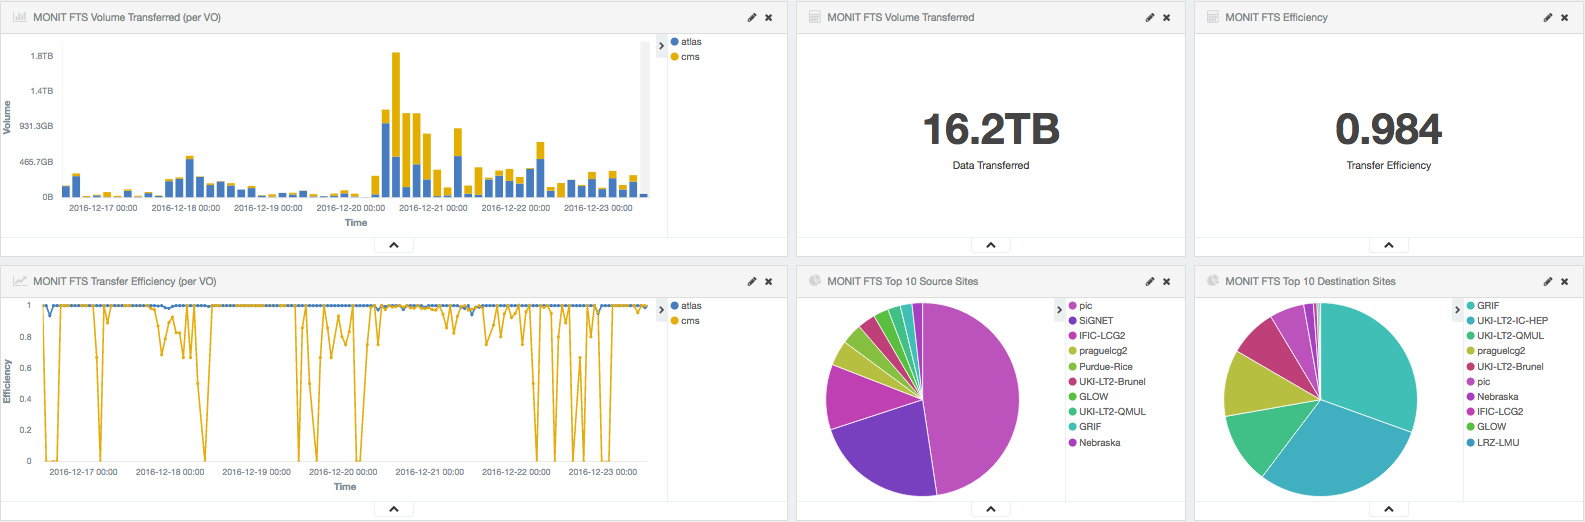
\includegraphics[width=\textwidth]{FTSIPv6Monitoring}
\caption{Figure showing a screenshot of the FTS monitoring dashboard.  It provides a summary of transfers over IPv6 in the week from December 17th to 23rd 2016}
\label{Fig:FTSMonitor}
\end{center}
\end{figure}

There are IPv4-only FTS services at RAL, BNL and Fermilab that are used by the LHC VOs.  Until they have been upgraded dual stack sites will have to use the CERN FTS service  if they want their transfers (where possible) to go over IPv6.  All the Tier-1s involved have indicated that they are likely to be able to upgrade their FTS service to dual-stack in the first half of 2017 and definitely by April 2018.


%\subsection{ETF test infrastructure}
%A separate IPv6-only ETF test infrastructure will need to be set up to
%monitor IPv6-ready sites. This must be done by April 2017.  This will
%be run in parallel to the production ETF test infrastructure. This
%service will provide sites with low level monitoring to help them
%identify problems with their IPv6 migration and not used for official
%availability metrics unless the site is providing some resources on
%IPv6-only. From April 2018 the official ETF infrastructure will be
%migrated to dual-stack. From this point on production work going over
%IPv6 should be considered entirely normal. This will hopefully
%encourage sites to investigate IPv6 before April 2018.

% The ETF infrastructure is primarily hosted at CERN, which can easily make the existing production version dual-stack.  Work is ongoing to set 

\subsection{Frontier Service}
ATLAS and CMS both use the Frontier Service\cite{FrontierATLAS, FrontierCMS} to access
conditions data across the Grid. The Frontier service has three
components:
\begin{itemize}
\item Frontier client: This software is run by ATLAS and CMS jobs. It
  converts a conditions database query into an HTTP request. The
  Frontier Client was made IPV6 compliant in January 2016.
\item Squid proxy: Sites are expected to deploy squid servers to cache
  the conditions data requests. Squid 3 is IPv6 compliant.  
\item Frontier Launchpad: This converts the HTTP requests back into
  database queries which are then submitted to the conditions
  database.  The Launchpads also run a squid to provide an extra layer of caching. 
\end{itemize}
The Frontier client software was one of the last to be made IPv6 compliant.  While all new releases of the VO software will use it, older versions of VO software will not (by default) and this could theoretically cause problems in future if there is a need to analyse data using an old release.

At the time of writing none of the Frontier Launchpad services had been upgraded to dual-stack.  This is because although Squid 3 is IPv6 compliant there were various bugs in it that made its performance, in certain circumstances, unacceptable.  Work is ongoing to resolve these bugs in the Squid software.  

\subsection{Other Services}
There are several other services such as certificate authorities,
software repositories, the GOCDB/OIM, GGUS, VOMS, the ETF test infrastructure and the BDII. These
are not used directly by VO jobs but are needed when configuring the
site.  These services should be made dual-stack when possible and
ideally by April 2018 (although some services might not fall under the
WLCG banner). It will depend heavily on the site setup as to whether
the lack of IPv6 connectivity will cause problems. Problems will have
to be followed up by the HEPiX working group as they appear.


\section{LHC experiments' migration}
The following section details the ongoing work from the LHC experiments to
upgrade their services to allow jobs to run on IPv6-only CPU resources.

\subsection{ALICE}
Unlike the other LHC experiments, ALICE uses fully federated storage; any site
can access the storage element of another site if needed (reading,
writing and data transfers). Therefore in order to ensure all job
types can run on IPv6-only CPU all data needs to be accessible over
IPv6. Some data is stored on multiple sites and therefore it does not
necessarily mean all sites will need to be dual-stack. To support
IPv6, the site storage elements will need to run XRootD v.4. The central
ALICE Grid services have been tested to run on IPv6 and have been dual-stack for over a year. 
Currently $5\%$ of the SEs provided to ALICE are dual-stack mode, while $65\%$ are running XRootD 4.

\subsection{ATLAS}
The ATLAS workload management system is called PanDA \cite{Panda}.
Pilot factories generate generic 'pilot' jobs which are sent directly to CEs at
sites. Once these pilots are started by the batch system, they will
contact the central Panda server  (done via HTTP). They
will also contact the ATLAS distributed Data Management System (Rucio\cite{Rucio}) for file lookup (done via HTTP). 
Most ATLAS jobs access Conditions data using the Frontier service.

The pilot factories that submit jobs to CEs have been made dual-stack.  The Rucio nodes are being migrated to SL7 towards 
the end of 2016 and this will be an opportunity to make them dual-stack.  Work is ongoing to debug and upgrade the Panda server. ATLAS also use the ARC Control Tower (aCT) to submit jobs primarily to NorduGrid but potentially any sites running an ARC CE. This will also
need to be made dual-stack. ATLAS are working on making all these
services dual-stack by April 2017.

\subsection{CMS}
CMS use the job submission middleware, glideinWMS, to launch HTCondor
worker nodes and its major components (frontend and factory). These
have been validated as IPv6-compliant. Some glidein factories are
already deployed in dual-stack. HTCondor itself is fully
IPv6-compliant, but the collectors and schedds still need to be all
dual-stack in production in order to support IPv6-only worker nodes.
The glideinWMS Integration Testbed (ITB) has been configured to be fully
dual-stack and it is used to test job submission to a few sites which
have enabled IPv6 on their WNs.

The central services hub, cmsweb.cern.ch, has been validated for
dual-stack operation and its production instance is running in
dual-stack mode. The CMS-specific job management systems (WMAgent for
production and CRAB3 for analysis) have not yet been fully tested on
IPv6, but they are expected to work with little effort needed. In any
case, they do not need to be dual-stack for the foreseeable future,
as they interact only with other central services.

The data management system, PhEDEx, uses the Oracle client for
communication between local site agents and the central service. Tests
have not yet been done, but Oracle 12c fully supports IPv6. Dual-stack
operation will not be required anyway.

Some CMS jobs make use of an XRootD storage federation.  Currently only a very small fraction
of the data is accessible using XRootD or GridFTP via IPv6. The global
and regional redirectors are only partly on dual-stack.

CMS plans to immediately start upgrading all central services to
dual-stack, to be completed in principle by the end of Run II, but
likely much earlier. Services contacted by worker nodes (like
HTCondor) will be given priority and will aim to be done by April
2017. A campaign will be launched at the beginning of 2017 to
encourage Tier-2 sites to upgrade their storage systems to dual-stack.

%At the time of writing, only eleven CMS sites expose IPv6 addresses for their services.

\subsection{LHCb}
LHCb uses the DIRAC framework to submit jobs to the grid. DIRAC
officially supports IPv6 and some other VOs, who use DIRAC, are
already using a dual-stack service in production.  LHCb submits
generic pilot jobs to CEs as needed. When these pilots start on a WN,
they contact the LHCb DIRAC central services for available tasks (via
the dips protocol) which are then executed. If input data is needed,
they contact the relevant storages using the sites SRM to access
the data.\footnote{In future this will be updated to bypass the SRM and construct the file 
location automatically.} Production jobs typically retrieve / download the data to
the worker node, as they know exactly how much data is needed. User
jobs stream data from the storage directly.

Once the job is done, it will upload the output to a storage
location. If the default preferred location is not available, all
other possible locations (available for LHCb) are tried in turn until
successful and a request is set in the central services of LHCb to
transfer the file to the preferred location when possible. If no
%dpk location is available, the job ends up in status "failed", and could
location is available, the job ends up in status ``failed", and could
be resubmitted depending on the conditions.

LHCb jobs running on an IPv6-only WN will need access to the following
resources:
\begin{itemize}
\item LHCb's DIRAC central services
\item Storage services supporting LHCb
\item Optionally, one of six VO-boxes at LHCb Tier-1 sites
\end{itemize}
Currently there is one Tier-1 storage and one Tier-2D storage that
support LHCb in a dual-stack configuration.  All important LHCb central services have already moved to dual-stack machines and the rest will move soon.

\section{Summary}
The LHC experiments are committed to being able to work on the Grid over IPv6.
Much work still remains to be done to make this a reality.  The HEPiX
IPv6 working group has validated that all essential software is IPv6
compliant.  Software developers should consider IPv6 compliance a
standard requirement and the emphasis should be on them to test this.
All the VOs have analysed their workflows on the Grid and have
provided a list of services which they will need to make dual-stack.
While exact time lines have not been agreed the amount of work
required is sufficiently small that it should be achievable by April
2017 without significantly disrupting normal WLCG operations.

From April 2017 sites will be allowed to deploy IPv6-only CPU
resources. Sites wishing to deploy IPv6-only CPU must deploy
dual-stack storage if they provide it.  All sites are encouraged to
upgrade their storage to dual-stack.  From the contact the HEPiX IPv6
working group has with sites, we believe that there are at most one or
two sites that wish to urgently upgrade making up less than $2\%$ of
the pledged WLCG CPU resources.  Any site wishing to upgrade should be
in contact with the HEPiX IPv6 working group to ensure that the
inevitable teething problems are resolved promptly.  By April 2018 it
should be possible to deploy IPv6-only CPU resources with relative
ease and by the end of Run II enough sites should have upgraded their
storage to dual-stack to allow almost complete data availability via
federated XrootD over IPv6.


\section*{Acknowledgements}
The authors acknowledge the contributions to this work made by former members of the HEPiX IPv6 Working Group and other colleagues within WLCG. In particular we express our thanks to Raul Lopes and Simon Furber at Brunel University London for their efforts in the configuration and testing of dual-stack DPM and Argus from IPv6-only compute nodes.
We also thank Edgar Fajardo Hernandez from the University of California, San Diego for his work on the validation of IPv6 and glideinWMS for the CMS experiment. The authors also acknowledge the support and collaboration of many other colleagues in their respective institutes, experiments and IT Infrastructures, together with the funding received by these from many different sources. These include but are not limited to the following:

\begin{enumerate}

\item The Worldwide LHC Computing Grid (WLCG) project is a global collaboration of more than 170 computing centres in 42 countries, linking up national and international grid infrastructures. Funding is acknowledged from many national funding bodies and we acknowledge the support of several operational infrastructures including EGI, OSG and NDGF/NeIC.

\item EGI acknowledges the funding and support received from the European Commission and the many National Grid Initiatives and other members. The EGI-Engage project is co-funded by the European Commission (grant number 654142).

\end{enumerate}


\section*{References}
\begin{thebibliography}{10}
%\bibitem{CheapIPv6} https://www.mythic-beasts.com/servers/virtual

%\bibitem{ApplePolicy} https://developer.apple.com/news/?id=05042016a

%dpk - added ref to our working group web
%dpk - modified other refs to meet guidelines
\bibitem{ipv6wg} The HEPiX IPv6 Working Group web site is to be found at {\tt http://hepix-ipv6.web.cern.ch}

%dpk \bibitem{CHEP15} J Bernier \textit{et al.} 2015 The production deployment of IPv6 on WLCG. \textit{Journal of Physics: Conference Series}, \textbf{664} 052018
\bibitem{CHEP15} Bernier J {\it et al} 2015 The production deployment of IPv6 on WLCG \textit{J. Phys.: Conf. Ser.} \textbf{664} 052018

%dpk \bibitem{Panda} Fernando Barreiro Megino \textit{et al.} 2015 PanDA: Evolution and Recent Trends in LHC Computing, Procedia Computer Science, Volume 66, Pages 439-447, ISSN 1877-0509.
\bibitem{Panda} Barreiro Megino F {\it et al} 2015 PanDA: evolution and recent trends in LHC computing, \textit {Proc. Comp. Sci.}, \textbf{66}, 439-447, ISSN 1877-0509.

%dpk \bibitem{Rucio} Garonne, V., Vigne, R., Stewart, G., Barisits, M., Lassnig, M., Serfon, C., Goossens, L., Nairz, A. and Atlas Collaboration, 2014. Rucio–The next generation of large scale distributed system for ATLAS Data Management. \textit{Journal of Physics: Conference Series} \textbf{513} 042021

\bibitem{Rucio} Garonne V, Vigne R, Stewart G, Barisits M, Lassnig M, Serfon C, Goossens L, Nairz A and Atlas Collaboration 2014 Rucio - the next generation of large scale distributed system for ATLAS data management. \textit{J. Phys.: Conf. Ser.} \textbf{513} 042021

%dpk \bibitem{perfSONAR}  P. Marcu, D. Schmitz, A. Hanemann and S. Trocha, 2010 Monitoring and visualisation of the Large Hadron Collider optical private network, \textit{9th RoEduNet IEEE International Conference, Sibiu, Romania}, pp. 316-321.
\bibitem{perfSONAR}  Marcu P, Schmitz D, Hanemann A and Trocha S  2010 Monitoring and visualisation of the Large Hadron Collider optical private network, \textit{9th RoEduNet IEEE International Conference, Sibiu, Romania}, pp. 316-321.

%dpk \bibitem{Stratum1} J Blomer \textit{et al.}; 2012 Status and future perspective of CernVM-FS \textit{Journal of Physics: Conference Series} \textbf{396} 052013
\bibitem{Stratum1} Blomer J {\it et al} 2012 Status and future perspective of CernVM-FS \textit{J. Phys.: Conf. Ser.} \textbf{396} 052013

%dpk \bibitem{FrontierCMS} Barry Blumenfeld \textit{et al.} 2012 Operational Experience with the Frontier System in CMS. \it{Journal of Physics: Conference Series}, \textbf{396} 052014
\bibitem{FrontierCMS} Blumenfeld B {\it et al} 2012 Operational experience with the frontier system in CMS \textit{J. Phys.: Conf. Ser.} \textbf{396} 052014

%dpk \bibitem{FrontierATLAS} D Barberis \textit{et al.} 2012 Evolution of grid-wide access to database resident information in ATLAS using Frontier. \textit{Journal of Physics: Conference Series}, \textbf{396} 052025  
\bibitem{FrontierATLAS} Barberis D {\it et al} 2012 Evolution of grid-wide access to database resident information in ATLAS using frontier \textit{J. Phys.: Conf. Ser.} \textbf{396} 052025 

%dpk \bibitem{DynaFed} Fabrizio  Furano,  \textit{et al.} 2012  Dynamic federations:  storage aggregation using open tools and protocols. \textit{Journal of Physics: Conference Series}, \textbf{396} 032042
\bibitem{DynaFed} Furano F  {\it et al} 2012  Dynamic federations:  storage aggregation using open tools and protocols \textit{J. Phys.: Conf. Ser.} \textbf{396} 032042

\end{thebibliography}

\end{document}
